\documentclass[11pt,a4paper]{article}
\usepackage[T1]{fontenc}
\usepackage[utf8]{inputenc}
\usepackage[margin=2.5cm]{geometry}
\usepackage{lmodern,microtype}
\usepackage{amsmath,booktabs,tabularx,graphicx}
\usepackage[round,authoryear]{natbib}
\usepackage[hidelinks]{hyperref}
\title{From GeoAI to environmental impact assessment: A systematic review of uncertainty continuity and digital twin architecture for the circular built environment}
\author{Author list and affiliations to be confirmed}
\date{Working manuscript v0.2 --- 2 November 2026}
\begin{document}
\maketitle
\begin{abstract}
Assessments of circular building material flows connect observations of the built environment with material inventories, temporal outflows, recovery pathways and environmental consequences. Uncertainty analysis within these individual tasks does not by itself establish continuity of uncertainty across their interfaces. This review is being developed to investigate which information is transferred, transformed or omitted between these tasks, and which digital twin capabilities could address documented interface limitations. Its analytical design connects three evidence streams: uncertainty in building material-flow assessments, domain-specific digital twin implementations, and transferable architectural mechanisms from interdisciplinary digital twin research. The intended contribution is an evidence-traceable architecture in which each component and connection responds to an identified requirement and is distinguished as directly demonstrated, synthesized across studies or newly proposed. Spatial boundaries, temporal validity, physical entities and decision interfaces serve as architectural dimensions. This initial manuscript establishes the research questions and synthesis protocol; corpus-wide eligibility assessment and architectural validation remain incomplete. Consequently, it does not report a final included-study count or claim an empirically validated end-to-end architecture.
\end{abstract}
\noindent\textbf{Keywords:} circular built environment; material flow analysis; uncertainty propagation; digital twin; architecture synthesis; evidence traceability.
\section{Introduction}
Building material-flow assessment requires several linked transformations. Observed building attributes are translated into material quantities; inventories are combined with temporal assumptions to estimate future flows; released materials are assessed for circular pathways; and these pathways are translated into environmental consequences. These transformations are supported by different modelling traditions. Probabilistic material-intensity characterization, dynamic material-flow analysis and circularity--life-cycle assessment provide complementary capabilities, but they do not necessarily establish the same evidential or probabilistic connection between their outputs and inputs \citep{U03,U12,U19}.

The relevant distinction is between the presence of uncertainty analysis and the continuity of uncertainty information. A downstream model may accept an upstream central estimate while disregarding its uncertainty. Alternatively, it may introduce a new uncertainty distribution without specifying whether it represents inherited error, additional process uncertainty or a scenario assumption. In either case, uncertainty at the final output cannot automatically be interpreted as a complete account of upstream uncertainty. The preliminary evidence audit therefore separates transfer status, representation change and changes in uncertainty magnitude rather than treating them as interchangeable outcomes.

The analytical chain used in this review comprises five stages: S1, observation and inference of building attributes; S2, material characterization and stock estimation; S3, temporal stock dynamics and material release; S4, recoverability and circular routing; and S5, environmental assessment and decision consequences. These are organizing categories for the review, not universal software layers. Studies can span several stages, bypass a stage or address only one transformation. Their actual variable relationships must therefore be examined alongside their initial stage assignments.

Digital twins are investigated here as a possible architectural response to interface limitations. Their contribution cannot be inferred from terminology, three-dimensional representation or the coexistence of several models. The review instead examines explicit capabilities for entity linkage, evidence integration, state updating, model coupling and interpretation of dependent outputs. Whether these capabilities preserve uncertainty or improve decisions is an empirical question for extraction, not an assumed benefit of digitization.

The intended contribution is a synthesized architecture whose components and connections can be traced to evidence and documented gaps. The research questions are:
\begin{enumerate}
\item What uncertainty information is transferred, transformed or left unassessed at the interfaces between S1--S5?
\item Which domain-specific digital twin capabilities implement these interfaces, and what limitations are reported or remain unresolved?
\item Which interdisciplinary mechanisms can address these limitations, under what transfer conditions, and with what level of supporting evidence?
\item How can these findings be synthesized into an architecture that accommodates spatial, temporal, physical and decision contexts without claiming universal applicability?
\end{enumerate}

\section{Related work and conceptual foundations}

Understanding circular material opportunities in the built environment requires connecting information that is normally produced for different purposes. Spatial observations describe buildings, stock models estimate their material content, dynamic models estimate future releases, and recovery and environmental assessments evaluate what those releases might mean for subsequent use. Integrated studies provide a basis for examining this connected workflow. Mastrucci et al. (2017) link geospatial characterization of building material stocks with life cycle assessment of end-of-life scenarios, while Ajayebi et al. (2020) address the spatial and temporal quantification of structural products for a prospective circular economy. Pei et al. (2024) review the techniques and tools connecting building material stock analysis and urban-scale life cycle assessment. These contributions establish integration as a substantive research problem, although their system boundaries and treatment of individual transformations differ \citep{I36,I37,I35}.

Comparison of these workflows motivates five analytical activities: observing and inferring building characteristics (S1), estimating material stocks (S2), modelling stock change and material outflows (S3), evaluating recovery and subsequent use (S4), and assessing environmental consequences and supporting decisions (S5). The labels are the organizing vocabulary of this review, rather than a five-stage architecture attributed to every cited study. They make it possible to compare equivalent transformations across different modelling traditions. Some studies combine activities, omit a transition, or iterate between them. Earlier geospatial frameworks also should not be retrospectively described as GeoAI implementations. GeoAI extends the observational part of this workflow through methods for interpreting spatial information, while geospatial and image-based demolition-waste modelling illustrates the connection between observation and material accounting \citep{I08,U01}.

The significance of this decomposition lies in the information exchanged at the boundaries. At S1--S2, observed or inferred characteristics must be associated with a building type, material composition or intensity coefficient. At S2--S3, an inventory becomes an estimate of when and how much material is released. Research on building-size--material-intensity relationships and the importance of lifespan assumptions illustrates why these are substantive modelling operations rather than neutral transfers of numbers \citep{I13,U11}. A downstream estimate may depend on the same uncertain classification or parameter as an upstream estimate. Treating those estimates as independent can therefore change the meaning of the combined assessment.

The next boundary introduces a different question: an estimated outflow is not necessarily an available secondary resource. Material-passport research examines information for end-of-life management, while probabilistic reusability assessment addresses the technical suitability of components \citep{I20,I21}. These approaches locate information needs between release and subsequent use. Recovery conditions, separation, quality and allocation to a reuse or recycling route need to be represented before environmental consequences can be interpreted. Studies comparing environmental assessment methods for component reuse further show the importance of how subsequent use is represented \citep{I22}. S3--S4 and S4--S5 are consequently useful analytical boundaries even where one model calculates several of these activities together.

Uncertainty must be interpreted within this chain of transformations. Michiels and Geeraerd (2020) distinguish incomplete knowledge from variability when examining how these influences are propagated and visualized in life cycle assessment \citep{I25}. For this review, the distinction matters because variation among buildings, uncertainty about an inferred building attribute and alternative future recovery scenarios do not have interchangeable meanings. A probability distribution, an interval, a set of scenarios and a qualitative data-quality description also communicate different kinds of information. An assessment may quantify uncertainty carefully within one model without preserving that representation when its output becomes another model's input.

We use uncertainty continuity to describe the traceable retention or explicit revision of uncertainty information, relevant dependencies and conditions of validity across such transformations. This is an analytical construct of the present review, not a claim that existing studies use a common term or that uncertainty must remain numerically unchanged. Propagation may alter an output distribution; new observations may support updating; aggregation may change the spatial support; and a recovery decision may convert a continuous quantity into an eligibility category. Conversely, an interval may be replaced by a point estimate, or the provenance needed to interpret it may not be reported. The relevant distinction is whether this change is documented and usable downstream. Missing reporting alone does not demonstrate that information was lost in the actual implementation.

Digital twins provide a related body of research on connections between physical entities, digital representations and updating processes. Jones et al. (2020) characterize the concept through a systematic literature review, while Boje et al. (2020) develop directions for semantic construction twins \citep{I27,I26}. Construction-focused reviews examine applications and enabling technologies \citep{I28,I29}. Together, these studies make it useful to examine the functions associated with a digital twin, rather than infer capabilities from its name. A geometric model may represent an asset without maintaining a data connection; an updated representation may support monitoring without implementing probabilistic propagation; and a conceptual architecture may describe services that have not been demonstrated operationally.

Definition differences are particularly relevant to the built environment. Abdelrahman et al. (2025) compare definitions and components across domains and distinguish high-performance real-time twins from long-term decision-support twins \citep{I31}. Their analysis cautions against treating real-time operation, bidirectional exchange and predictive functionality as equally mature or universally required across applications. For material-flow assessment, the appropriate update may occur after a survey, renovation or change in recovery conditions. The methodological question is whether the timing and content of that update preserve the validity of the connected assessment, not simply whether a continuous sensor stream exists.

Research on uncertainty-aware twins offers mechanisms for investigating this question. Kapteyn et al. (2021) formulate coupled asset--twin dynamics using a probabilistic graphical model and demonstrate calibration and updating in an aircraft-related application \citep{I33}. Lin et al. (2021) review uncertainty quantification and software risks in digital-twin-based management and control \citep{I32}. These studies support examination of probabilistic state representation, dependencies and updating as architectural capabilities. They do not establish that the same mechanisms already provide uncertainty continuity from building observation to circular material decisions. Their relevance must be assessed against the entities, quantities, temporal processes and validation conditions of the target workflow.

The three bodies of literature therefore meet at the interfaces between activities. Material-flow studies identify the quantities and transformations that require continuity; uncertainty research explains what must be retained or revised; and digital-twin research offers ways to connect representations, observations and analytical services. Spatial scale, temporal validity and stakeholder information requirements condition these connections. The existence of a scalable software structure, for example, does not itself demonstrate that the underlying material assumptions remain valid across buildings, districts and regions. Similarly, a dashboard can communicate an uncertainty estimate without establishing how it was obtained or propagated.

Existing reviews provide complementary foundations: Pei et al. (2024) examine stock--LCA integration, Michiels and Geeraerd (2020) examine uncertainty and variability, and Abdelrahman et al. (2025) examine DT definitions and components \citep{I35,I25,I31}. The present review brings these perspectives into a common interface-based comparison. It asks which uncertainty-related connections are directly documented, which can be synthesized from compatible studies, and which remain proposals responding to identified limitations. The intended contribution is an evidence-traceable architectural synthesis. It does not presume that all transitions are missing from prior work, nor does it present a newly implemented or validated end-to-end digital twin.
\section{Materials and methods}

\subsection{Review design: a shared interface as the unit of synthesis}

The review connects evidence on material-assessment workflows, uncertainty and digital-twin capabilities through a shared analytical unit: a documented interface between activities. Search families provide complementary routes to this evidence, rather than separate reviews with unrelated conclusions. The design addresses four linked questions: which transformations connect S1--S5; what happens to uncertainty at those transformations; which DT capabilities are relevant under the reported conditions; and how the findings support an evidence-traceable architecture. PRISMA 2020 guides reporting of study selection and PRISMA-S guides documentation of searches \citep{M01,M02}. These reporting guidelines do not replace the extraction and synthesis procedures specified below.

For publication p and interface i$\rightarrow$j, the extraction record is E(p,i,j) = {entity, input, transformation, output, uncertainty-in, uncertainty-out, dependencies, DT-function, context, evidence}. Entity identifies the building, component or material represented; context includes spatial support, temporal validity and information-user requirements; evidence contains the publication identifier and page, section, equation or figure locator. DT-function is recorded as not applicable or not reported where appropriate. Thus a non-DT material-flow study and a DT mechanism study can be compared through an explicit information requirement without claiming that they implement the same system. Figure 1 shows this connected workflow; Figure 2 specifies the analytical joins.

\subsection{Information sources and search families}

The database searches cover Scopus, Web of Science Core Collection and IEEE Xplore. Base, also denoted S, refers to stage-specific building/material-flow searches. U denotes uncertainty and DT denotes digital twin. The domain families are Base, Base+U, Base+DT and Base+DT+U. General DT and DT+U searches provide definition and transferable-mechanism evidence, with their non-domain origin retained. Supplementary searches for integrated workflows are not restricted by publication year or publisher. Exact filters are documented per search execution rather than assumed identical across historical runs.

Scopus searches use TITLE-ABS-KEY; Web of Science searches use Topic, which also includes Keywords Plus. IEEE field selections and split-query variants are retained in the execution records. The logical search structure is Q(i,k) = B(i,k) AND S(i) AND optional(U) AND optional(DT), where k identifies the query version. The version index matters because some historical DT searches use a broader domain block than earlier Base searches. The logical diagram is therefore not evidence that every historical query forms a strict subset of one identical Base query.

Table 1 lists the concepts used to organize retrieval. The complete archived strings, including exclusions and database adaptations, remain in Supplement S1 and the recovered S1--S3 query files. Missing historical execution details are flagged in the audit rather than reconstructed as executed searches. New explanatory examples in this section are not presented as additional database searches.

\begin{center}\small\begin{tabularx}{\linewidth}{XX}\toprule
Block & Search concepts and examples\\\addlinespace
Domain B & building stock*, existing building*, built environment, material cadastre*, resource cadastre*\\\addlinespace
S1 & GeoAI, remote sensing, computer vision, LiDAR, point cloud*, building geometry, building classification\\\addlinespace
S2 & material stock*, material inventor*, material intensit*, material composition, building archetype*, quantity takeoff\\\addlinespace
S3 & material flow*, dynamic stock*, stock turnover, service life, building lifetime*, demolition timing, material outflow*\\\addlinespace
S4 & reuse, recycl*, recover*, deconstruction, urban mining, disassembl*, secondary material*, reverse logistics\\\addlinespace
S5 & life cycle assessment, embodied carbon, environmental impact*, carbon footprint, decision support\\\addlinespace
DT & "digital twin" OR "digital twins"\\\addlinespace
U & uncertaint*, probabil*, stochastic*, Bayesian, "Monte Carlo", sensitiv*, variabil*, calibrat*, robust*, prediction/confidence intervals\\\addlinespace
\bottomrule\end{tabularx}\end{center}

For clarity, the four domain combinations are B AND S(i); B AND S(i) AND U; B AND S(i) AND DT; and B AND S(i) AND DT AND U. General DT+U omits the building-stage restriction. Broad U terms improve retrieval but do not establish uncertainty analysis: sensitivity, calibration or robustness must be interpreted from the methods. Membership is recorded at publication level after deduplication. Actual overlaps are calculated from identifiers, not inferred from query labels or summed database counts \citep{M02}.

\subsection{Eligibility, deduplication and selection}

Each publication is screened against its intended evidential role. Domain studies must describe a relevant activity or transformation in building-material assessment. U evidence must identify an affected quantity, assumption or decision and explain its treatment; a generic uncertainty statement is insufficient for a mechanism claim. DT evidence must describe representations, data connections, updating or analytical functions. Architecture papers can provide conceptual evidence without being relabelled operational implementations. External-domain mechanisms and secondary reviews are retained separately as complementary evidence. A paper need not address all five stages or demonstrate successful uncertainty continuity to be relevant.

Original database exports are preserved. DOI values are normalized; records without DOI are checked using native identifiers and bibliographic information. Similar titles, conflicting DOIs and related conference/journal versions require adjudication. Duplicate publications are distinguished from multiple reports of one study. Multiple search memberships are retained without multiplying the unique-publication denominator.

Selection proceeds through identification, deduplication, title/abstract screening, full-text retrieval, full-text eligibility and inclusion. Full text is checked for identity, completeness and methodological detail. Abstract-only material and incomplete previews do not support full-text mechanism extraction. Reports that cannot be obtained or adequately assessed do not enter the final synthesis. Their records remain in the selection audit: non-retrieval is distinguished from exclusion after assessment, and available but unread reports remain pending rather than being assigned a scientific exclusion reason. No target number of included publications is imposed.

Full-text exclusions have a primary reason, with secondary notes where needed: outside the material-flow domain; no relevant DT function for a DT-specific synthesis; no substantive U treatment for a U-specific synthesis; or insufficient methodological evidence for the intended analytical role. A report can be ineligible for the strict triple intersection while remaining relevant to a complementary stream. Reasons and evidence locators are preserved. PRISMA reporting follows these distinctions \citep{M01}.

\subsection{Interface extraction and uncertainty coding}

Stage assignment is based on the operation actually performed. An edge S(i)$\rightarrow$S(j) requires a documented use of an upstream output in a downstream activity; mentioning two stages does not establish an edge. Non-adjacent links and feedback are retained. Table 2 defines the common questions applied across the four adjacent interfaces. These are extraction prompts, not findings that every study implements the listed transformations.

\begin{center}\small\begin{tabularx}{\linewidth}{XXXX}\toprule
Interface & Transformation to inspect & Uncertainty information to trace & Candidate DT function to investigate\\\addlinespace
S1$\rightarrow$S2 & Observations/attributes to material quantities & Classification uncertainty, geometry, material intensities and their dependencies & Identity, semantic mapping, provenance and data-quality representation\\\addlinespace
S2$\rightarrow$S3 & Inventory to time-dependent release & Inventory uncertainty, lifetimes, survival and scenario dependencies & State/time representation, linked dynamic models and versioning\\\addlinespace
S3$\rightarrow$S4 & Released material to recoverable supply & Timing, condition, separation yield, quality and route eligibility & Condition updates, component tracking and recovery-service linkage\\\addlinespace
S4$\rightarrow$S5 & Recovery routes to impacts/decision & Yield, substitution, allocation, impact factors and joint assumptions & Assessment-service coupling, scenario provenance and decision communication\\\addlinespace
\bottomrule\end{tabularx}\end{center}

The extraction distinguishes uncertainty source, nature, representation and operation. Parameter, model and scenario uncertainty are recorded separately from spatial/temporal variability where the study permits this distinction \citep{I25}. Representations include distributions, samples, intervals, scenarios and qualitative quality statements. Dependencies include reported covariance, correlation, shared parameters and explicit independence assumptions. Missing dependence information is not coded as independence.

The interface state uses non-exclusive operation codes: transferred, transformed, updated, newly introduced, or demonstrably discarded. A separate reporting status identifies insufficient description. Reduced uncertainty requires a stated comparison and metric; improved prediction accuracy alone does not establish reduction. Source statements are distinguished from reviewer interpretation. Each mechanism claim requires a locator and a short evidence note. Scale, temporal resolution, update trigger, validity period and stakeholder information roles are extracted as conditions of the interface, not as disconnected descriptive categories.

\subsection{Linking interface requirements to DT capabilities}

DT coding records the authors' definition, physical referent, digital representation, data connection, update direction/frequency, analytical service and demonstrated maturity \citep{I27,I26,I31}. Real-time operation and bidirectional control are not imposed as universal requirements. Nor is a BIM/GIS model automatically treated as an operational DT. The distinction between probabilistic modelling and demonstrated asset--twin updating is informed by uncertainty-aware DT research \citep{I33,I32}.

For each interface, an evidence chain links: observed limitation $\rightarrow$ information requirement $\rightarrow$ reported DT capability $\rightarrow$ compatibility conditions $\rightarrow$ supported architectural connection. Compatibility is checked against the entity, variable meaning, unit, spatial support, temporal horizon and dependency representation. For example, a general-domain Bayesian updating mechanism is not assigned to S3--S4 merely because both involve uncertainty; the proposed connection must explain what recovery-related state would be updated, by which observation and under which assumptions. If that connection is inferred across studies, it is explicitly coded as synthesis rather than a demonstrated domain implementation.

\subsection{Relational analysis and architectural synthesis}

The same interface records generate three connected matrices: interface $\times$ uncertainty operation; interface $\times$ DT capability; and DT capability $\times$ uncertainty operation. Every populated cell resolves to supporting publication and evidence identifiers. A fourth join table links all three dimensions and records whether the connection occurs within one study or is synthesized across studies. No complete S1--S5 chain is inferred simply by concatenating unrelated papers. Figure 2 shows the shared record that prevents the three matrices from becoming independent analyses.

For a given eligible corpus C, the cell count is n(i,u,d) = the number of distinct publications in C supporting interface i, uncertainty operation u and DT capability d together. Direct within-publication counts and cross-study synthesis are reported separately; inferred links do not inflate empirical frequencies. Coverage of a coded property is its distinct supporting-publication count divided by the number of eligible, assessed publications for that analysis. The denominator and unreported cases accompany each figure. Multilabel coding means marginal totals can exceed the unique-publication total. This treatment follows the need to distinguish study counts from category participation, illustrated in Falsafi et al. (2025) \citep{M03}.

Descriptive outputs include evidence heatmaps, overlap plots and interface networks. A line represents a coded connection, not causality; thickness represents a specified count, not effectiveness. Temporal counts summed across databases are labelled database occurrences unless record-level deduplication supports unique-publication counts. Statistical tests are not assumed valid for overlapping categories, and visual differences are not labelled significant without an appropriate test design. Heterogeneous outcomes are not pooled in an effectiveness meta-analysis.

Architectural elements are classified as directly supported, synthesized from compatible studies, or proposed in response to a documented gap. The architecture thus links each module and connection to its evidential basis and to the interface requirement it addresses. A reported limitation, missing reporting and an absence in the retrieved corpus remain distinct. The resulting structure is a review-based conceptual synthesis; operational effectiveness and cross-scale generalization require subsequent validation.

\subsubsection{Transition-level evidence and continuity distribution (D01)}

The adjacent-boundary set is B={B12,B23,B34,B45}, corresponding to S1$\rightarrow$S2, S2$\rightarrow$S3, S3$\rightarrow$S4 and S4$\rightarrow$S5. O5 (other inputs$\rightarrow$S5) is retained outside this set. A paper with S5 outputs is not automatically assigned B45: its upstream recovery input must be documented. The existing analysis unit is a unique publication--context pair a=(p,b), not an independent study or a physical material flow. Scenario variants within that pair are not counted again. A future scenario-level extraction would require a new unit and denominator.

The archived continuity codebook assigns one primary status c(a): Q, discussion/review; N, downstream transfer not demonstrated; R, inputs prepared for propagation; S, sensitivity/representation comparison; P, partial or incompletely documented transfer; E, quantified outputs for selected uncertain inputs. These are evidence categories, not an ordinal maturity scale. In particular, E does not establish transport of every upstream uncertainty or dependency. The R code here is distinct from the reported-function R code used for DT features.

D01 is computed as n(b,c)=sum over a of 1[b(a)=b and c(a)=c]. Its margins satisfy N(b)=sum\_c n(b,c) and sum\_b N(b)=|A|. Ribbon width is proportional to n(b,c); it encodes the distribution of assessments into evidence states, not the magnitude of uncertainty transferred. All four adjacent boundaries remain in the exported table, including zero cells. A zero for B34 means no counted assessment in this selected extraction, not absence of relevant research. Multiple pairs from one publication remain dependent. No downstream continuity is inferred by joining different publications into a synthetic S1--S5 trajectory.

To adjudicate an actual transition, extraction must identify the upstream uncertain variable X, its representation U(X), the documented mapping Y=f(X,theta), and the downstream use of U(Y). For stochastic propagation, samples, joint distributions or an equivalent dependence treatment must be traceable through f; a sensitivity plot alone is not such evidence. Updating is separately recorded when new observations change the inferred state or parameter distribution. The notation describes what is inspected in the papers; this review does not itself simulate material stocks or perform Bayesian updating. An interval on Y without a documented connection to upstream X supports output-UQ evidence but not necessarily end-to-end continuity \citep{I25,I33}.

\subsubsection{Stage–function incidence network (D02)}

For each publication p, stage s and function f, x(p,s,f)=1 only when the source coding contains a reported-function state R. C denotes conceptual/proposed/review support and NR denotes no positive recorded feature. R is not independent validation or proof of an operational whole-system twin. The weighted bipartite network has w(s,f)=sum\_p x(p,s,f); stage-node counts are the distinct union of supporting publications across functions, and function-node counts are the corresponding union across stages. Repeated tags within a publication--stage--function cell must be collapsed before aggregation.

Only S1--S5 cells enter the network; X-coded adjacent construction, scheduling or cost functions remain outside it. Edge width is proportional to w. In the archived plotting implementation, stage-node area is 220+55N(s) points squared and function-node area is 170+45N(f), so node size is an affine visual encoding, not a strictly proportional area encoding. The network is an incidence map without inter-stage direction. Even if the same paper supports S2 and S3, a transition is counted only after its input--mapping--output connection is separately evidenced. D02 supplies candidate functions for the transition join; it does not substitute for that join.

\subsubsection{Exact positive-code configurations (D03)}

For the non-review DT--U subset, each publication is represented by z(p)=(z1,...,z7), where zk=1 for a reported R-coded mechanism and 0 otherwise. The seven dimensions are probabilistic representation, Bayesian state/parameter inference, explicit dependency transport, residual/shift diagnostics, online adaptation, interval-coverage assessment and uncertainty-linked alerts/actions. The original C and NR states are preserved separately: zero in this projection does not establish absence. Publications assigned to the review/reference-architecture family are omitted from this configuration analysis.

For each observed binary pattern v, its exact-intersection frequency is h(v)=sum\_p 1[z(p)=v]. Each publication contributes to exactly one pattern, and sum\_v h(v)=N. Marginal mechanism frequency is m(k)=sum\_v v(k)h(v). Columns are sorted by decreasing h, then number of positive codes, with a deterministic binary-pattern tie-break. This is an UpSet-style exact-set display, not clustering, a maturity ranking or an inferred causal sequence. Identical positive-code patterns do not establish identical implementations; implementations may differ in context and in their C/NR states.

\subsubsection{Source–method associations within the same transition context (D04)}

Source and method labels are joined on the compound key (publication\_id, context), never on publication alone. Let A(q) be the set of counted pairs carrying source q and A(m) those carrying method m. The cell count is n(q,m)=|A(q) intersection A(m)| and the row denominator is N(q)=|A(q)|. Colour encodes P(m|q)=100 n(q,m)/N(q), while bubble area is 150 n(q,m) points squared. Empty source rows have an undefined percentage, not zero. Rows and columns are ordered by their assessment frequencies, with codebook order resolving ties.

Because labels are multilabel, percentages within a row need not sum to 100\%. The join establishes co-occurrence within one assessed context, not that the method was specifically applied to that source. For example, a context containing two sources and two methods yields four co-occurrence cells; a source-specific treatment claim requires an additional explicit evidence relation. Source labels are not automatically mapped to epistemic or aleatory uncertainty. Prediction-error diagnostics and scenario comparison are not automatically probabilistic propagation.

\subsubsection{Joining the four outputs into transition-based architectural evidence}

D01 establishes the recorded continuity state of a boundary; D04 identifies accompanying sources and methods; D02 locates reported domain functions; D03 provides general-DT mechanism configurations. The architectural join uses the boundary record as its anchor and stores: boundary\_id, material variable and unit, uncertainty source/representation, continuity state, method, DT function, update trigger, spatial/temporal validity, evidence locator and support class. Within-publication links are distinguished from compatible cross-study synthesis and proposed additions. General DT configurations are not relabelled S1--S5 implementations.

For each boundary, the results will report the assessed publication count, context count, distribution of continuity states, documented variable transformations, candidate DT functions and the evidential status of each proposed connection. A transition diagram can therefore show what is preserved, transformed, newly introduced or insufficiently reported without interpreting a stage--function edge as uncertainty transport. Missing B34 coverage remains visible. A conceptual missing link is not filled by reallocating O5 assessments to B45 or by treating a review as an independent experiment.

\subsubsection{Verification and limits of the current analytical inputs}

The aggregation audit independently reconstructs D01 cells from context records, D02 weights from R-coded cells, D03 exact memberships from mechanism codes and D04 intersections from source/method assignments. It checks unique keys, ID sets, marginal conservation, row denominators and source-file hashes. The current snapshot reproduces 23 contexts from 20 publications, 16 positive stage--function edges, nine exact configurations across ten non-review records, and 46 positive cells in the 100-cell source--method matrix. These are analysis-subset counts, not PRISMA included-study totals.

This arithmetic check does not reread or validate the semantic interpretation of every paper. Some archived extraction anchors refer to earlier coding tables rather than page-specific primary evidence. Such cases require evidence-locator completion and compatibility checks against the current eligibility ledger before submission. The figures are therefore reproducible from the archived coding, but are not certified as a newly completed full-text synthesis. No statistical independence, inter-reviewer agreement or significance test is inferred from successful reproduction.

\subsection{Evidence appraisal, traceability and reporting status}

Appraisal considers data provenance, explicit assumptions, dependency treatment, validation, scenario conditions and reproducibility. Synthetic demonstrations, empirical tests and conceptual proposals are distinguished. A universal numerical quality score is not imposed on heterogeneous designs. The decision ledger retains source, role, eligibility reason and evidence locator, while code and count inputs accompany figures. The review does not claim an independent two-human-reviewer process where none is documented.

Figure 3 is an audit-status PRISMA-style diagram for the broad Base+DT+U search, not a completed all-scenario selection flow. Its counts are read from the archived decision ledgers. Figure 4 reports adjudication within the previously selected focused sets; these are subsets with overlapping membership, not additional independent searches. The broader Base, Base+U, Base+DT and general-DT workflows cannot yet be labelled complete through Included. Pending reports are excluded from current substantive synthesis but remain visible as pending in the audit. Completion of those decisions is required before replacing these status diagrams with final submission-ready PRISMA flows. This status statement is editorial and must be updated when the review is closed, rather than removed while the work remains incomplete.\begin{figure}[p]\centering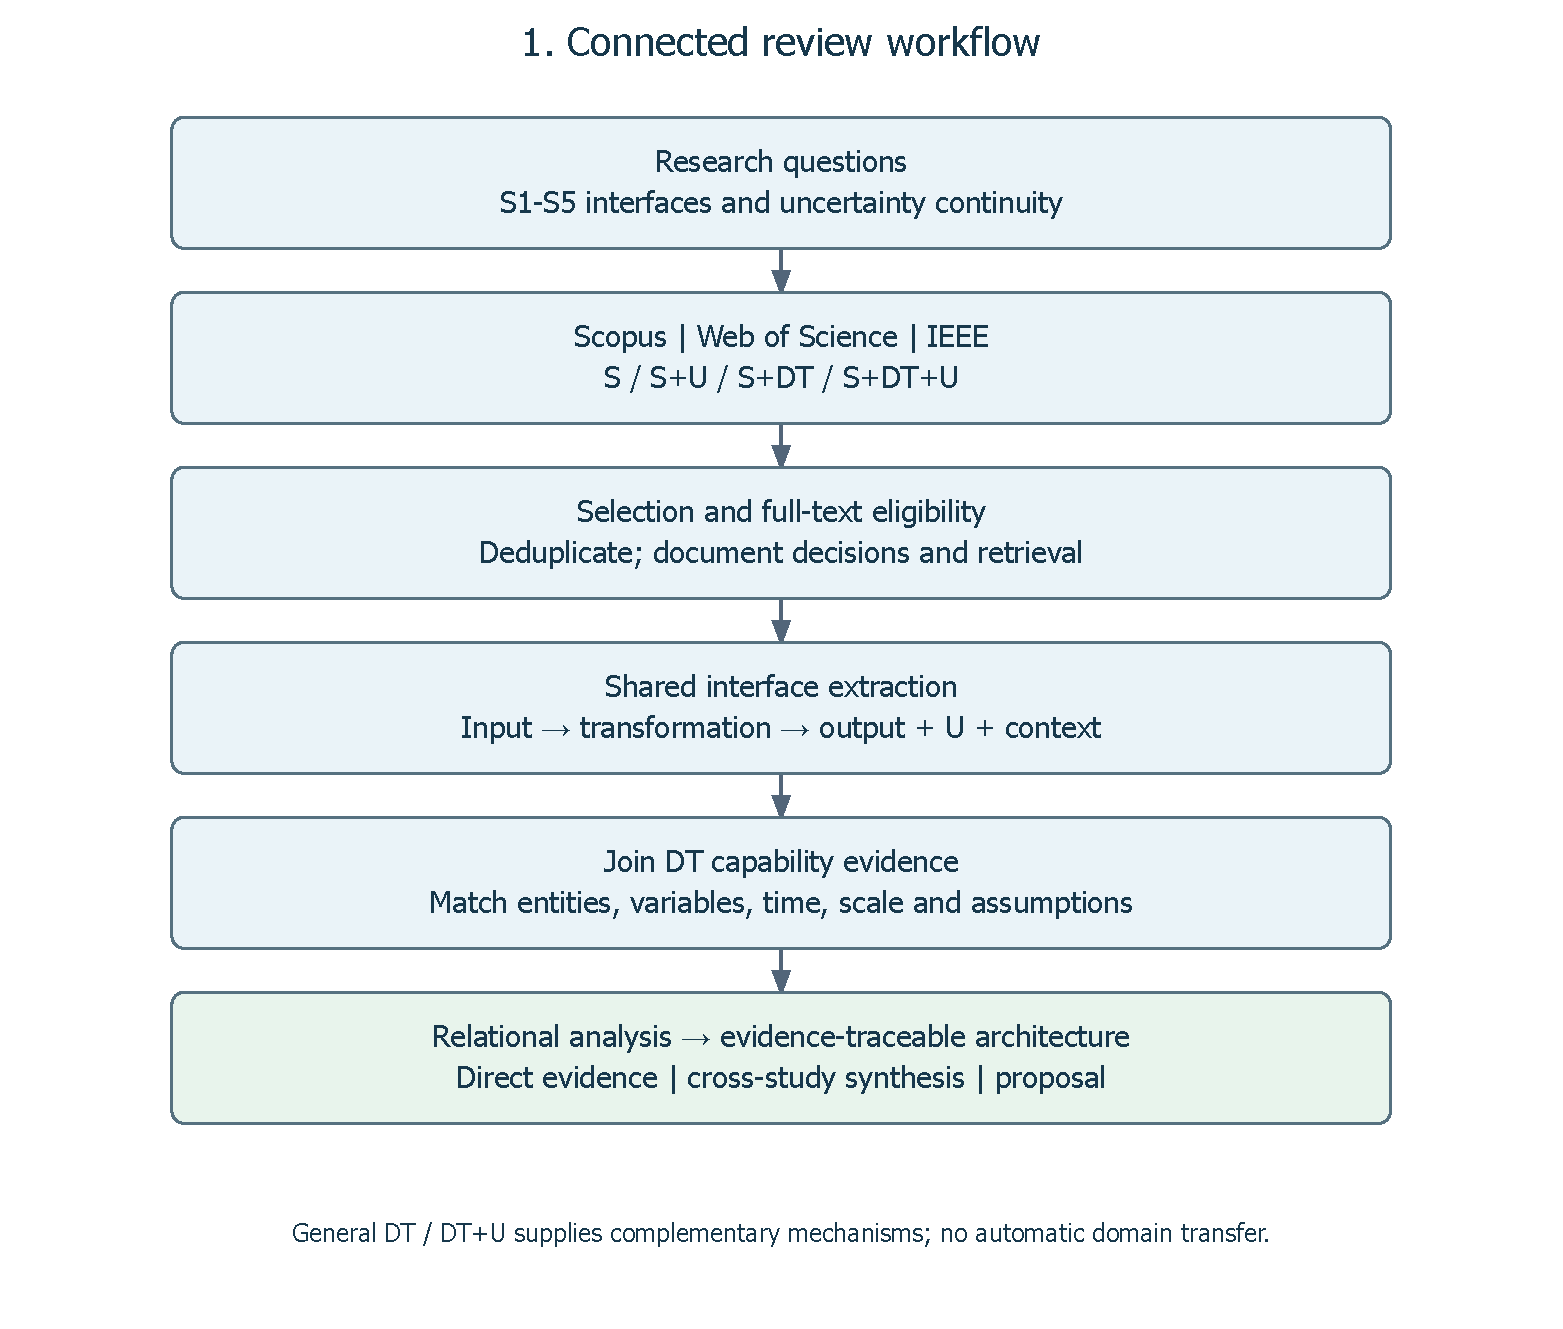
\includegraphics[width=\linewidth]{figures/methods/workflow_en.pdf}\caption{Connected review workflow.}\end{figure}
\begin{figure}[p]\centering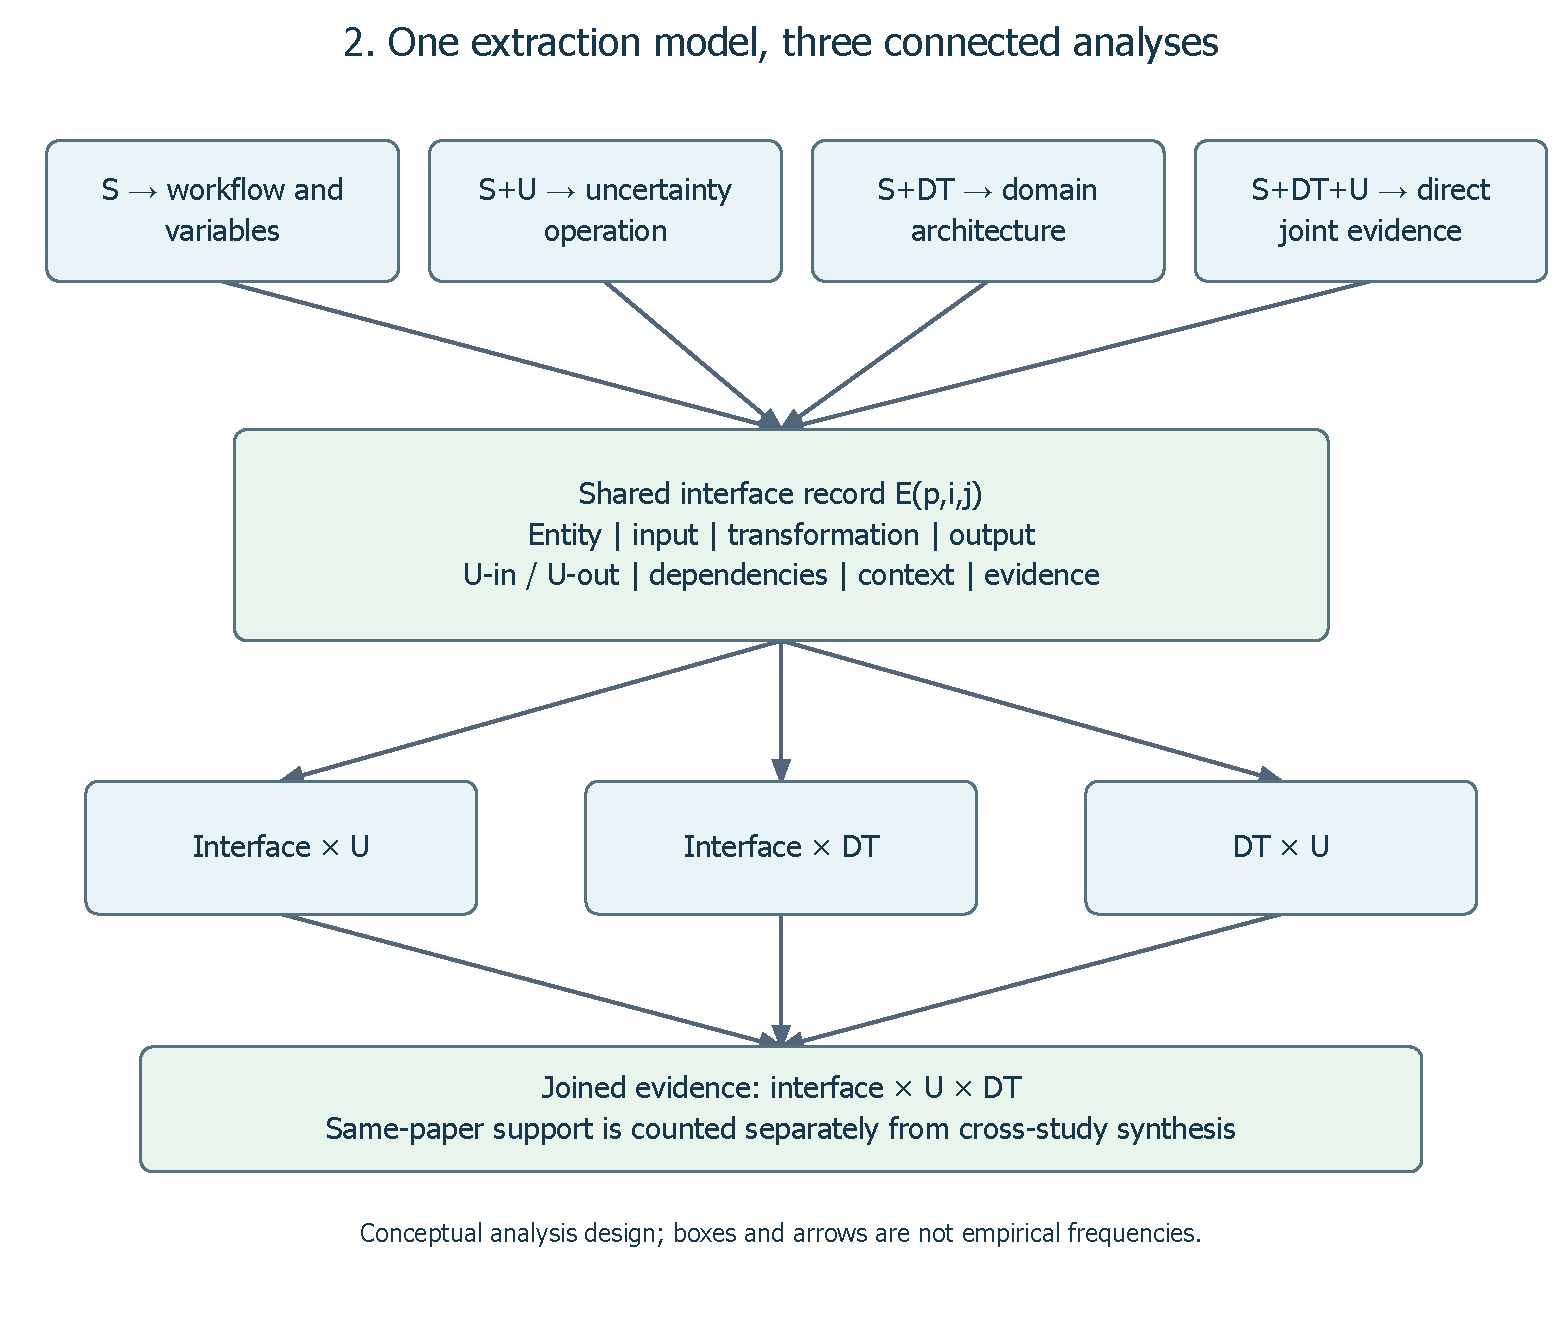
\includegraphics[width=\linewidth]{figures/methods/evidence_join_en.pdf}\caption{Shared interface records connect the three relational analyses.}\end{figure}
\begin{figure}[p]\centering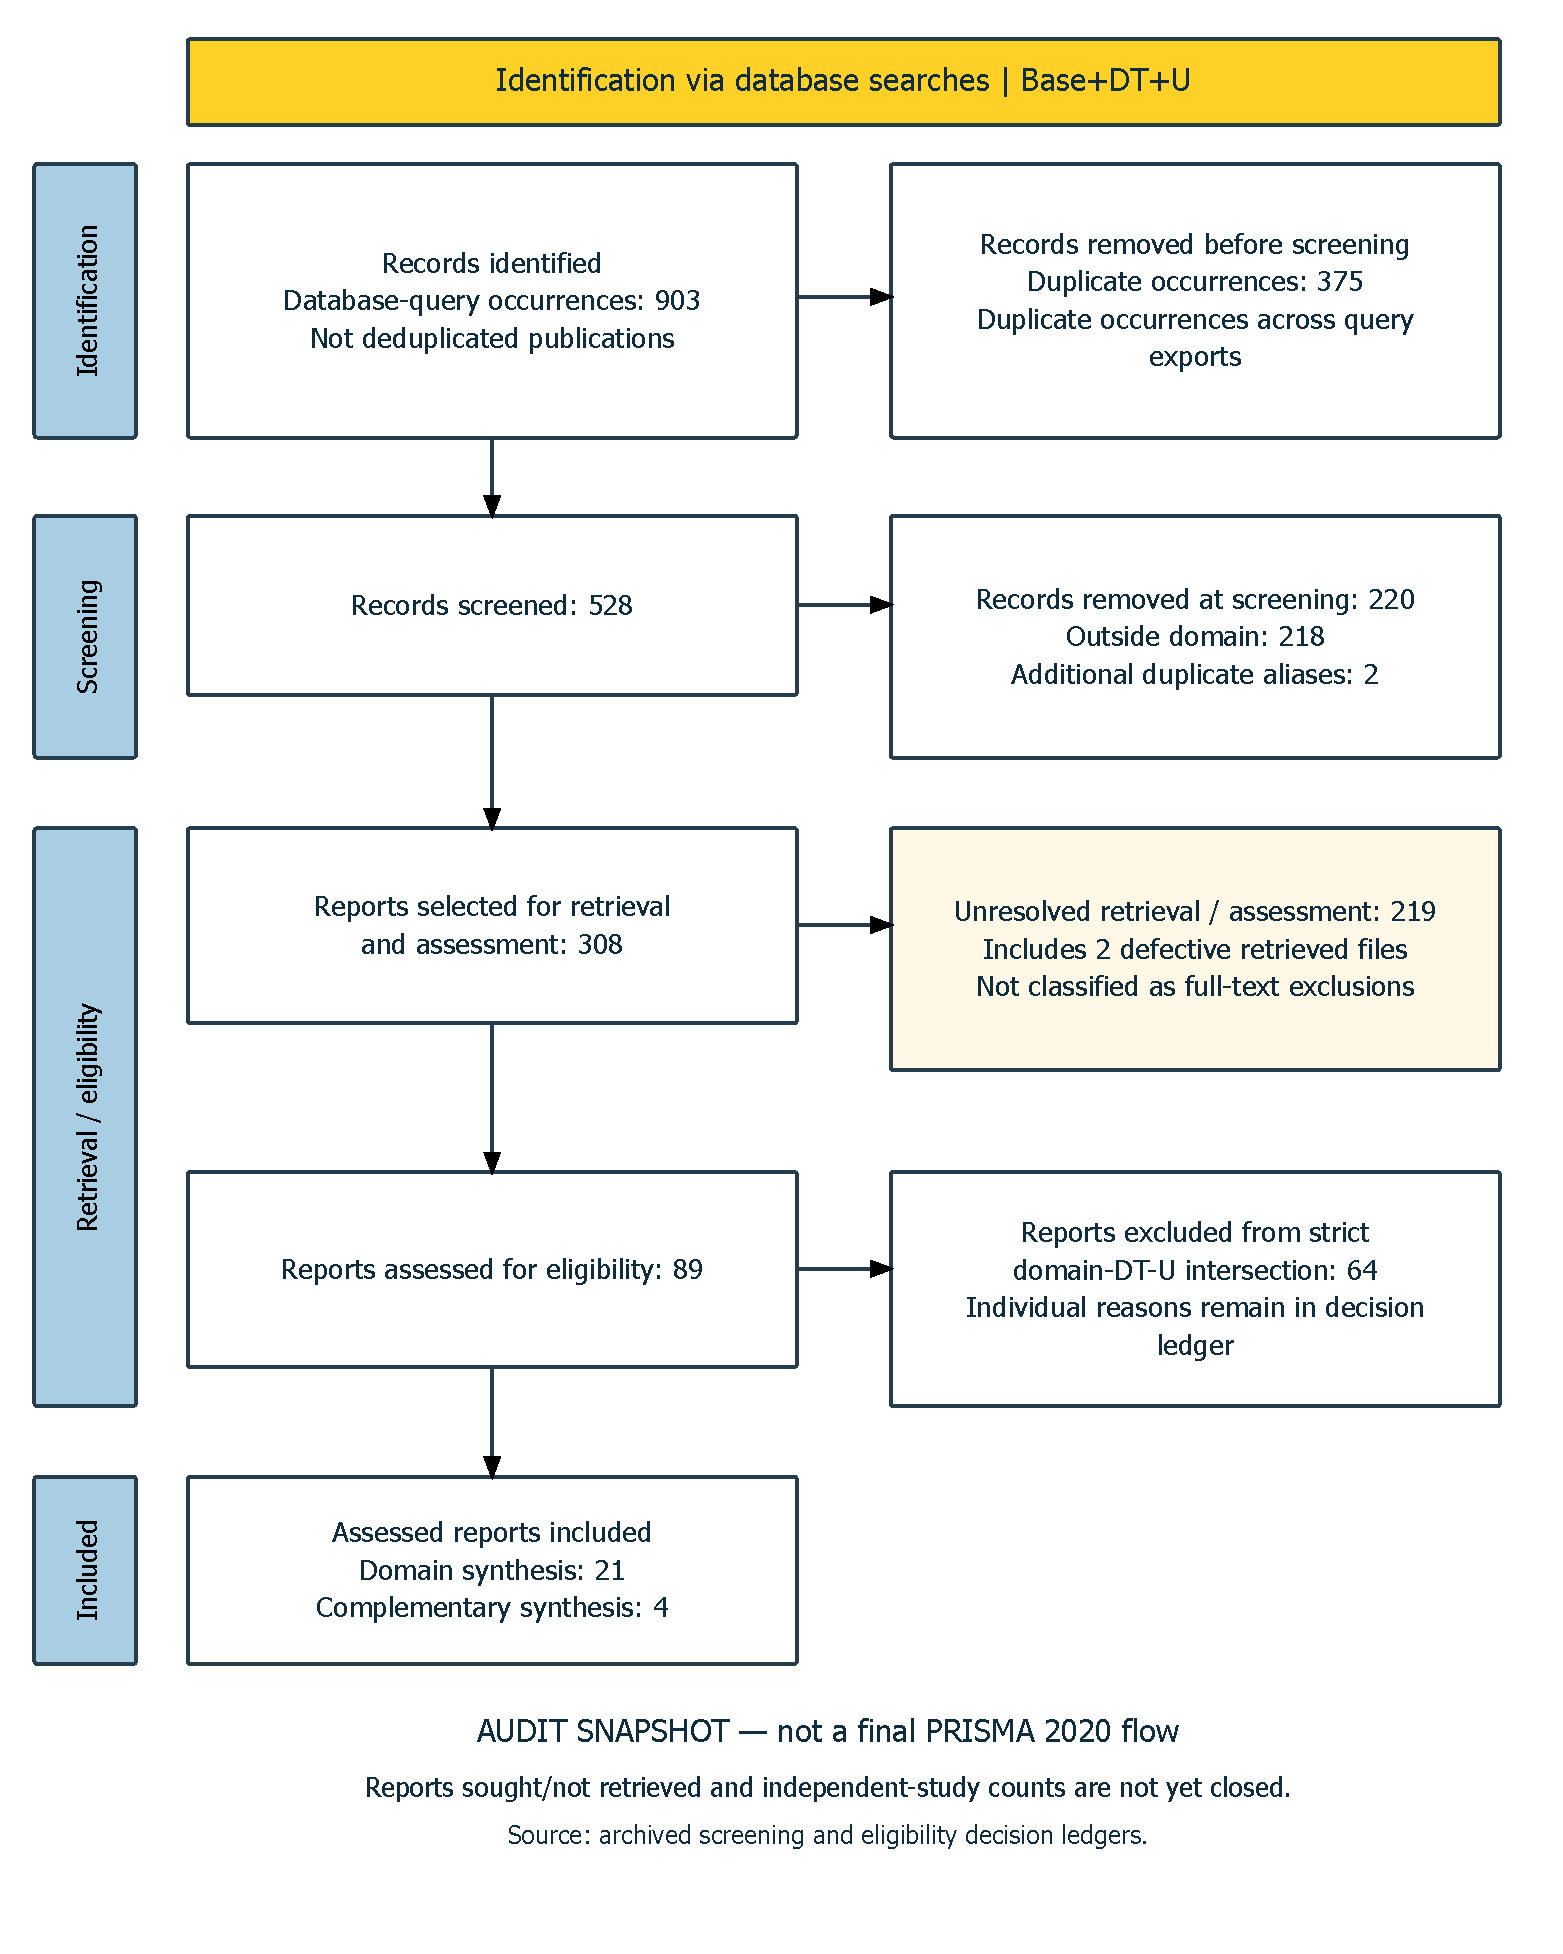
\includegraphics[width=\linewidth]{figures/methods/prisma_broad_dtu_status_en.pdf}\caption{Broad Base+DT+U audit status; not a final PRISMA flow.}\end{figure}
\begin{figure}[p]\centering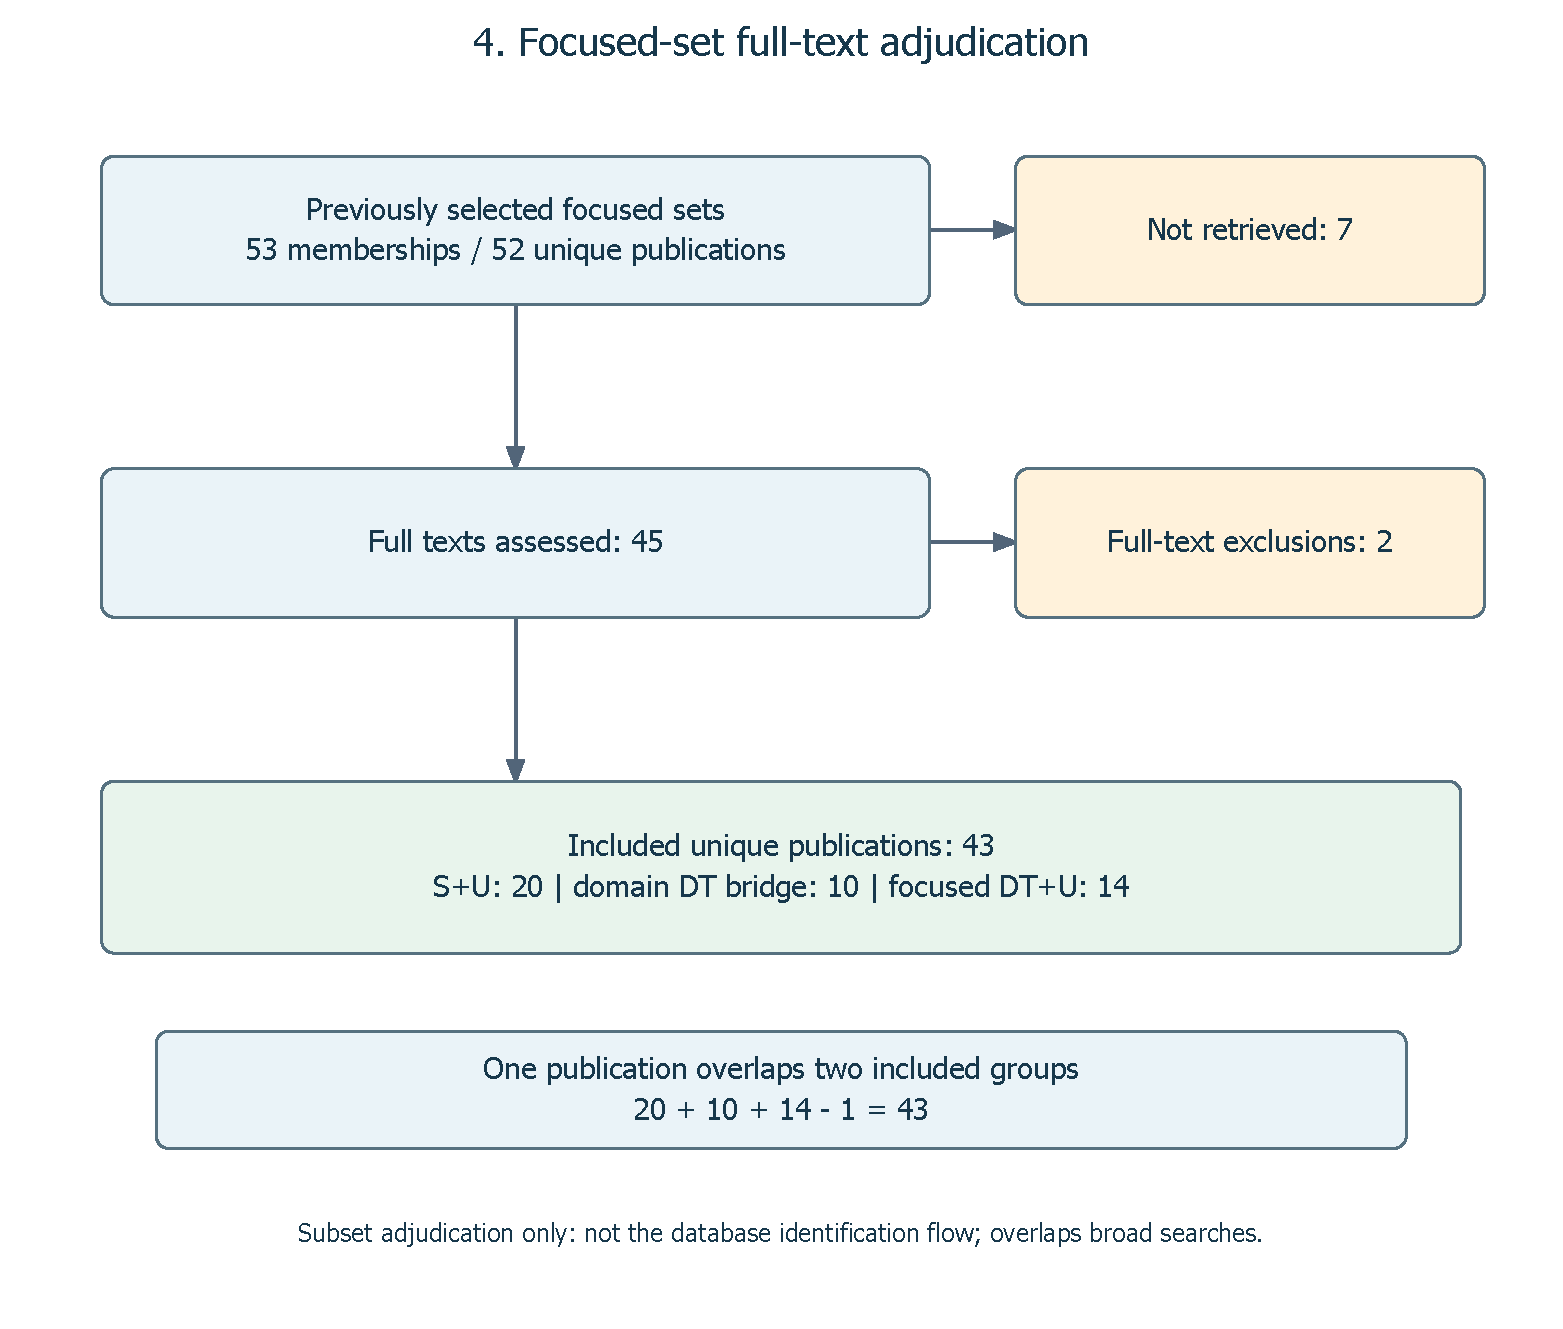
\includegraphics[width=\linewidth]{figures/methods/focused_selection_status_en.pdf}\caption{Focused-set adjudication only; not a database-wide selection flow.}\end{figure}

\section{Preliminary interface evidence}
This section reports bounded observations from the existing extraction, not final corpus-wide results. The current 21-record working set combines 18 retained candidates from the earlier S1--S3 audit with three subsequent S4--S5 studies. It includes methodological and complementary evidence, and is not a set of 21 demonstrations of uncertainty continuity.

\subsection{Building attributes to material quantities}
The semisupervised material-intensity study provides probabilistic representations that can support downstream stock modelling \citep{U03}. This capability is distinct from demonstrating that classification uncertainty and quantity uncertainty are jointly propagated through a complete inventory. The feature-based stock estimation audit identifies a further distinction between reported predictive error and uncertainty retained during aggregation of point estimates \citep{U05}. These observations motivate separate extraction of parameter uncertainty, prediction uncertainty and the aggregation rule.

\subsection{Material stocks to temporal flows}
The lifespan study examines the sensitivity of stock and demolition accounts to lifetime assumptions, while the probabilistic dynamic MFA study explicitly connects uncertain inputs with stock and flow outputs \citep{U11,U12}. This interface changes the temporal allocation of material quantities. Its uncertainty cannot be characterized solely by the accuracy of the total stock: flow timing and spatial aggregation can alter the relevance of lifetime assumptions. These studies provide useful mechanisms for the synthesis, without establishing that every upstream observation error has been retained.

\subsection{Recovery and environmental consequences}
The multicycle renovation framework links reuse feasibility and recovery-related inputs with circularity and environmental assessment \citep{U19}. The extraction distinguishes shared inputs and compatible scenarios from a fully specified joint stochastic transfer between the branches. The circularity score is not itself an input passed into LCA. The reported Monte Carlo calculations do not document all distributional dependencies or paired draws needed to reproduce a complete cross-branch uncertainty chain.

Damage-to-environmental-impact studies provide complementary mappings between physical states, interventions and carbon consequences \citep{U20,U21}. They cannot automatically be treated as evidence for uncertain material recovery yields. Within the current working set, the S3--S4 connection remains insufficiently established for a claim of continuous uncertainty propagation from released quantities to recoverable quantities and quality. This is a bounded finding, not evidence that the wider literature contains no such mechanism.

\subsection{Domain-specific DT evidence}
The broader S1--S5 DT retrieval and the narrower uncertainty-gated DT retrieval are separate corpora. Their screening does not yet support a final architecture-frequency analysis or a validated domain-wide gap map. This subsection will be developed from interface-level full-text extraction rather than from keyword occurrence or retrieval counts. Candidate architectures will be assessed for entity linkage, model coupling and actual update behavior before their capabilities are attributed to a functioning twin.

\section{Architecture synthesis: analytical specification}
\subsection{Synthesis principle}
The architecture will be derived from documented requirements, rather than by adding independently desirable capabilities to a generic layer diagram. Each component and connection must identify the gap it addresses, its mechanism of operation, its evidence provenance and its limits. The specification below defines the synthesis task; it is not a validated final architecture.

\begin{table}[htbp]
\centering\small
\caption{Architectural dimensions to be populated from evidence. These are synthesis categories, not established findings.}
\begin{tabularx}{\textwidth}{@{}p{0.25\textwidth}X@{}}
\toprule
Dimension & Structural question \\
\midrule
Entities and relations & Which buildings, components, materials, events and flows are represented, and how are their identities related? \\
Evidence and state & How are observations, inferred properties and scenario choices distinguished and updated? \\
Transformation interfaces & Which model maps each input to an output, with what uncertainty and dependency assumptions? \\
Space and time & How are aggregation, spatial support, temporal validity and event changes represented? \\
Decision interface & How are information requirements and objectives connected to interpretable outputs? \\
Evidence traceability & Which source supports each capability and connection, and where does the review introduce a new proposal? \\
\bottomrule
\end{tabularx}
\end{table}

\subsection{Uncertainty continuity as an interface property}
For an interface with uncertain input $X$, additional parameters $\theta$ and output $Y=g(X,\theta)$, continuity requires an explicit account of how information about $X$ and its dependencies enters the calculation of $Y$. This does not require one universal numerical technique. Joint sampling, analytical propagation, interval methods and scenario branching support different information types. A method must not create a probability distribution where only qualitative or scenario evidence exists.

\subsection{Proposed evaluation conditions}
The synthesized architecture should be evaluated against explicit interface tests: preservation of material identity and units; consistency of aggregation and mass balance; handling of shared uncertain causes; traceability of the outputs affected by a state update; and visibility of unresolved uncertainty. These are proposed evaluation conditions. Their empirical implementation and the selection of a demonstrative case remain future work for this manuscript.

\section{Discussion and limits of the intended contribution}
The intended contribution is a structural synthesis connecting documented uncertainty-interface requirements with demonstrated or transferable digital twin capabilities. Traceability of evidence supports the rationale for a proposed architecture; it does not establish the architecture's effectiveness. Claims of uncertainty reduction require comparable before-and-after evidence. Claims of decision improvement require evaluation of decision consequences. Neither follows automatically from richer metadata or a more detailed digital representation.

Multi-scale representation, consistency across scale transitions and computational scalability are distinct properties. Likewise, storing timestamps, updating a state and revising downstream predictions are distinct temporal capabilities. The final synthesis must identify which properties are supported and which remain proposed. It must also preserve the distinction between literature silence and a demonstrated technical limitation.

\section{Concluding research position}
The developing review treats uncertainty continuity as a property of connected transformations rather than a count of uncertainty methods. Its architecture will be constructed through an explicit chain from source evidence to interface limitation, structural requirement and candidate mechanism. At this stage, the manuscript establishes that analytical direction and records preliminary evidence. Final conclusions await completion of the domain-specific DT synthesis and reconciliation of the supporting evidence streams.

\bibliographystyle{elsarticle-harv}
\bibliography{references}
\end{document}
